\begin{name}
{Sở GD Bạc Liêu}
{ĐỀ THI THỬ TỐT NGHIỆP THPT--NĂM 2022 }
\end{name}
\Opensolutionfile{ans}[ans/sobaclieu]
\begin{ex} 
 Số phức liên hợp của số phức $z=-2+5 i$ là
\choice
{$\bar{z}=5-2 i$}
{$\bar{z}=2+5 i$}
{$\bar{z}=2-5 i$}
{\True $\bar{z}=-2-5 i$}
\end{ex}

\begin{ex} % Câu 2
 Trong không gian với hệ trục tọa độ $O x y z$, biết điểm $M(1; a; b)$ thuộc đường thẳng $\Delta: \dfrac{x-2}{1}=\dfrac{y+2}{2}=\dfrac{z-1}{-1}$. Giá trị của $a+b$ bằng
\choice
{$3$}
{$2$}
{$-1$}
{\True $-2$}
\end{ex}

\begin{ex} % Câu 3
 Trong không gian với hệ trục tọa độ $O x y z$, cho mặt phẳng $(\alpha): 2 x+3 z-1=0$. Vectơ nào dưới đây là một vectơ pháp tuyến của $(\alpha)$ ?
\choice
{\True$\vec{n}=(2; 0; 3)$}
{$\vec{n}=(2; 3;-1)$}
{$\vec{n}=(2; 0;-3)$}
{$\vec{n}=(2; 3; 0)$}
\end{ex}

\begin{ex} % Câu 4
 Ông A gửi $100$ triệu đồng tiết kiệm với lãi suất $5,5 \%$ trên một năm và tiền lãi hàng năm được nhập vào vốn đề tính lãi cho năm tiếp theo. Hỏi theo cách đó thì sau it nhất bao nhiêu năm ông A thu được số tiền cả gốc và lãi ít nhất là $200$ triệu đồng (biết rằng lãi suất không thay đổi)
\choice
{$13$ năm}
{\True $15$ năm}
{$14$ năm}
{$12$ năm}
\end{ex}

\begin{ex} % Câu 5
\immini[thm]{ Cho hàm số $y=f(x)$ có đồ thị như hình vẽ. Hàm số đã cho nghịch biến trên khoảng nào dưới đây?
\choice
{$(-1; 1)$}
{\True $(0; 1)$}
{$(-2;-1)$}
{$(-1; 0)$}
}
{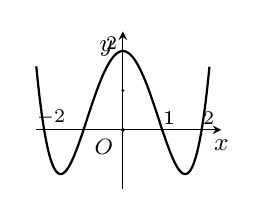
\begin{tikzpicture}[scale=.5]
\draw[-stealth] (-2.2,0) -- (2.5,0) node[below]{\small $x$};
\draw[-stealth] (0,-1.5) -- (0,2.5) node[below left]{\small $y$};
\draw[thick,smooth,samples=100] plot[domain=-2.2:2.2](\x,{.5*(\x)^4-2.5*(\x)^2+2});
\draw [fill=white,draw=black] (0,0) circle (1pt)node[below left]{\footnotesize $O$};
\foreach \x in{-2,1,1,2}\draw(\x,0) circle (.5pt) node[shift={(60:5pt)}]{\scriptsize $\x$};
\foreach \y in{2,}\draw(0,\y) circle (.5pt) node[shift={(145:5pt)}]{\scriptsize $\y$};
\end{tikzpicture}}
\end{ex}

\begin{ex} % Câu 6
 Xét $I=\int_{0}^{1}(x-1) e^{x^{2}-2 x+3} \mathrm{~d} x$, nếu đặt $u=x^{2}-2 x+3$ thì ta được tích phân nào sau đây?
\choice
{$I=-\int_{2}^{3} e^{u} \mathrm{d} u$}
{\True $I=-\dfrac{1}{2} \int_{2}^{3} e^{u} \mathrm{d} u$}
{$I=\int_{2}^{3} e^{u} \mathrm{d} u$}
{$I=\dfrac{1}{2} \int_{2}^{3} e^{u} \mathrm{d} u$}
\end{ex}

\begin{ex} % Câu 7
 Có bao nhiêu cách sắp xếp 5 học sinh thành một hàng ngang?
\choice
{$5^{5}$}
{5}
{$C_{5}^{5}$}
{\True $5!$}
\end{ex}

\begin{ex} % Câu 8
 Tập nghiệm $S$ của bất phương trình $3^{x}<9$ là
\choice
{$S=(2;+\infty)$}
{$S=[2;+\infty)$}
{$S=(-\infty; 2]$}
{\True$S=(-\infty; 2)$}
\end{ex}

\begin{ex} % Câu 9
\immini[thm]{ Hàm số nào dưới đây có đồ thị như đường cong trong hình vẽ bên dưới? 
\choice
{$y=x^{4}+2 x^{2}-1$}
{\True $y=x^{3}-2 x-1$}
{$y=-x^{3}+2 x-1$}
{$y=x^{2}-2 x-1$}
}{
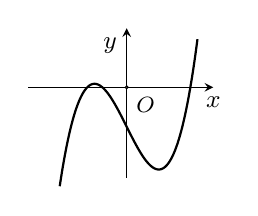
\begin{tikzpicture}[scale=.5]
\draw[-stealth] (-2.5,0) -- (2.2,0) node[below]{\small $x$};
\draw[-stealth] (0,-2.3) -- (0,1.5) node[below left]{\small $y$};
\draw[thick,smooth,samples=100] plot[domain=-1.7:1.8](\x,{(\x)^3-2*(\x)-1});
\draw [fill=white,draw=black] (0,0) circle (1pt)node[below right]{\footnotesize $O$};

\end{tikzpicture}
}
\end{ex}

\begin{ex} % Câu 10
 Trong không gian với hệ trục $O x y z$, cho điềm $A(1;-2; 3)$ và mặt phẳng $(P): 2 x+m y-(2 m-1) z+3=0$. Tìm giá trị của tham số $m$ để điểm $A$ thuộc mặt phẳng $(P)$ ?
\choice
{$m=-1$}
{\True$m=1$}
{$m=2$}
{$m=0$}
\end{ex}

\begin{ex} % Câu 11
 Cho khối cầu có bán kính $r=4$. Thể tích khối cầu đã cho bằng
\choice
{$\dfrac{256 \pi}{3}$}
{\True$\dfrac{64 \pi}{3}$}
{$256 \pi$}
{$64 \pi$}
\end{ex}

\begin{ex} % Câu 12
 Cho hàm số $f(x)=2 \sin 2 x$. Trong các khẳng định sau, khẳng định nào đúng?
\choice
{$\int f(x) \mathrm{d} x=-\dfrac{1}{2} \cos 2 x+C$}
{\True $\int f(x) \mathrm{d} x=-\cos 2 x+C$}
{$\int f(x) \mathrm{d} x=\dfrac{1}{2} \cos 2 x+C$}
{$\int f(x) \mathrm{d} x=\cos 2 x+C$}
\end{ex}

\begin{ex} % Câu 13
 Số nghiệm của phương trình $\log _{2}(x-3)+\log _{2}(x-1)=3$ là
\choice
{3}
{0}
{\True $1$}
{2}
\end{ex}

\begin{ex} % Câu 14
 Đường tiệm cận đứng của đồ thị hàm số $y=\dfrac{1-x}{x+1}$ là
\choice
{$y=1$}
{$x=1$}
{$y=-1$}
{\True$x=-1$}
\end{ex}

\begin{ex} % Câu 15
 Cho biết $\int_{1}^{2} f(x) \mathrm{d} x=2$. Giá trị của $\int_{1}^{2} 4 f(x) \mathrm{d} x$ bằng
\choice
{\True 8}
{16}
{6}
{2}
\end{ex}

\begin{ex} % Câu 16
 Cho hình hộp có đáy là hình vuông cạnh bằng $a$ và chiều cao $3 a$. Thề tích của hình hộp đã cho bằng
\choice
{$a^{3}$}
{$\dfrac{1}{3} a^{3}$}
{\True $3 a^{3}$}
{$9 a^{3}$}
\end{ex}

\begin{ex} % Câu 17
 Cho khối chóp có diện tích đáy $B=12 a^{2}$ và chiều cao $h=5 a$. Tính thể tích $V$ của khối chóp.
\choice
{\True $V=20 a^{3}$}
{$V=80 a^{3}$}
{$V=60 a^{3}$}
{$V=10 a^{3}$}
\end{ex}

\begin{ex} % Câu 18
 Cho khối nón có bán kính $r=4$ và chiều cao $h=2$. Thể tích của khối nón đã cho bằng
\choice
{$8 \pi$}
{$32 \pi$}
{$\dfrac{8 \pi}{3}$}
{\True$\dfrac{32 \pi}{3}$}
\end{ex}

\begin{ex} % Câu 19
 Với $a$ là số thực dương tùy ý, $\log \left(10 a^{2}\right)$ bằng
\choice
{$1+(\log a)^{2}$}
{$10 \log a$}
{\True$1+2 \log a$}
{$20 \log a$}
\end{ex}

\begin{ex} % Câu 20
 Một lớp có $15$ học sinh nữ và $ 20$ học sinh nam. Chọn ngẫu nhiên $4$ học sinh tham gia trực tuần cùng Đoàn trường. Xác suất đề trong $4$ học sinh được chọn có không quá một nữ bằng 
\choice
{$\dfrac{3705}{5236}$}
{\True$\dfrac{57}{136}$}
{$\dfrac{855}{2618}$}
{$\dfrac{79}{136}$}
\end{ex}

\begin{ex} % Câu 21
 Trong không gian với hệ trục $O x y z$, đường thẳng $d$ đi qua điểm $M(1; 2; 3)$ và song song với trục $\mathrm{Oz}$ có phương trình là
\choice
{$d:\left\{\begin{array}{l}x=1+t \\ y=2+t,(t \in \mathbb{R}). \\ z=3\end{array}\right.$}
{\True $d:\left\{\begin{array}{l}x=1 \\ y=2 \\ z=3- t\end{array},(t \in \mathbb{R})\right.$}
{$d:\left\{\begin{array}{l}x=1 \\ y=2+t,(t \in \mathbb{R}). \\ z=3\end{array}\right.$}
{$d:\left\{\begin{array}{l}x=1+ t \\ y=2 \\ z=3\end{array},(t \in \mathbb{R})\right.$}
\end{ex}

\begin{ex} % Câu 22
 Cho cấp số nhân $\left(u_{n}\right)$ với $u_{1}=2$ và công bội $q=3$. Tính $u_{3}$.
\choice
{$u_{3}=54$}
{\True $u_{3}=18$}
{$u_{3}=12$}
{$u_{3}=6$}
\end{ex}

\begin{ex}% Câu 23
 Trong không gian với hệ trục $O x y z$, tọa độ tâm $I$ của mặt cầu $(S): x^{2}+y^{2}+z^{2}-2 x-4 y-6=0$ là
\choice
{$I(2; 4; 0)$}
{$I(1; 2; 3)$}
{$I(2; 4; 6)$}
{\True$I(1; 2; 0)$}
\end{ex}

\begin{ex} % Câu 24
 Cho hàm số $y=-x^{3}+3 x^{2}+1$. Khẳng định nào sau đây là đúng?
\choice
{Hàm số nghịch biến trên khoảng $(0; 2)$}
{Hàm số đồng biến trên khoảng $(-\infty; 0)$}
{\True Hàm số đồng biến trên khoảng $(0; 2)$}
{Hàm số đồng biến trên khoảng $(2;+\infty)$}
\end{ex}

\begin{ex} % Câu 25
 Với giá trị nào của tham số $m$ thì phương trình $3^{x}-1=m$ có nghiệm?
\choice
{\True $m>-1$}
{$m>1$}
{$m<1$}
{$m>0$}
\end{ex}

\begin{ex} % Câu 26
 Cho hàm số $y=f(x)$ có bảng biến thiên như sau:
 \\ \centerline{

\begin{tikzpicture}
\tkzTabInit[nocadre,lgt=1.2,espcl=2.2]
{$x$ /.6,$f'(x)$ /.6,$f(x)$ /1.5}
{$-\infty$,$0$,$3$,$+\infty$}
\tkzTabLine{,+,$0$,-,$0$,+,}
\tkzTabVar{-/ $-\infty$ ,+/$2$,-/$-4$,+/$+\infty$}
\end{tikzpicture}
}\\
Tổng giá trị cực tiểu và giá trị cực đại của hàm số đã cho bằng
\choice
{0}
{\True $-2$}
{2}
{3}
\end{ex}

\begin{ex} % Câu 27
 Cho số phức $z$ thỏa mãn $2 i z-5+i=i-(z-2 i)$. Môđun của số phức $w=z-1+i$ bằng
\choice
{$\dfrac{1}{5}$}
{$\sqrt{\dfrac{29}{5}}$}
{\True$\dfrac{9}{5}$}
{1}
\end{ex}

\begin{ex} % Câu 28
 Cho hàm số $y=f(x)$ có đạo hàm $f^{\prime}(x)=x(x-1)(x+1)^{4}, \forall x \in \mathbb{R}$. Hỏi hàm số đã cho có bao nhiêu điểm cực trị?
\choice
{\True 2}
{4}
{1}
{3}
\end{ex}

\begin{ex} % Câu 30
 Diện tích hình phẳng giới hạn bời hai đường $y=x^{2}-3$ và $y=x-3$ bằng
\choice
{$\dfrac{125}{6}$}
{\True$\dfrac{1}{6}$}
{$\dfrac{125 \pi}{3}$}
{$\dfrac{\pi}{6}$}
\end{ex}

\begin{ex}% Câu 31
 Họ tất cả các nguyên hàm của hàm số $f(x)=e^{x}+2$ là
\choice
{\True$\dfrac{e^{x+1}}{x+1}+2 x+C$}
{$\dfrac{1}{x} e^{x+1}+C$}
{$e^{x}+2 x+C$}
{$e^{x}+C$}
\end{ex}

\begin{ex} % Câu 32
 Cho hai số phức $z_{1}=1-2 i, z_{2}=x-4+y i$ với $x, y \in \mathbb{R}$. Tìm cặp $(x; y)$ để $z_{2}=2 \bar{z}_{1}$
\choice
{\True $(x; y)=(4; 6)$}
{$(x; y)=(6;-4)$}
{$(x; y)=(5;-4)$}
{$(x; y)=(6; 4)$}
\end{ex}

\begin{ex} % Câu 33
 Gọi $A, B, C$ lần lượt là các điểm biểu diễn của các số phức $z_{1}=2, z_{2}=4 i, z_{3}=2+4 i$ trong mặt phẳng tọa độ $O x y$. Diện tích của tam giác $A B C$ bằng
\choice
{\True 8}
{6}
{4}
{2}
\end{ex}

\begin{ex} % Câu 35
 Điểm nào dưới đây thuộc đồ thị hàm số $y=x^{4}+2 x^{2}-2$ ?
\choice
{Điểm $P(-1;-1)$}
{\True Điềm $Q(-1; 1)$}
{Điểm $M(-1; 0)$}
{Điểm $N(-1;-2)$}
\end{ex}

\begin{ex} % Câu 36
 Tập xác định của hàm số $y=\log _{4} x$ là
\choice
{$D=(-\infty;+\infty)$}
{$D=(-\infty; 0)$}
{\True $D=(0;+\infty)$}
{$D=[0;+\infty)$}
\end{ex}

\begin{ex} % Câu 37
 Trong không gian với hệ trục $O x y z$, cho điểm $A(2; 1;-5)$. Hình chiếu vuông góc của điềm $A$ trên trục hoành là
\choice
{$M(2; 0;-5)$}
{$M(0; 0;-5)$}
{$M(0; 1;-5)$}
{\True $M(2; 0; 0)$}
\end{ex}

\begin{ex} % Câu 38
 Số giao điểm của đồ thị hàm số $y=x^{3}+3 x^{2}+2$ và đường thẳng $y=4$ là
\choice
{0}
{\True 3}
{2}
{1}
\end{ex}

\begin{ex} % Câu 29
 Cho hình chóp $S. A B C$ có đáy $A B C$ là tam giác đều cạnh $a, S A$ vuông góc với mặt phẳng đáy và $S A=\dfrac{a \sqrt{3}}{2}$. Gọi $M$ là trung điểm cạnh $B C$, góc giữa $S M$ và mặt phẳng $(A B C)$ bằng
\choice
{$90^{\circ}$}
{\True $30^{\circ}$}
{$60^{\circ}$}
{$45^{\circ}$}
\end{ex}

\begin{ex} % Câu 34
 Cho hình chóp $S. A B C D$ có đáy $A B C D$ là hình chữ nhật, biết $A B=a, A D=a \sqrt{2}, S A$ vuông góc với mặt phẳng đáy và $S A=a$. Khoảng cách từ $A$ đến mặt phẳng $(S B D)$ bằng
\choice
{$\dfrac{a \sqrt{2}}{5}$}
{$\dfrac{a \sqrt{3}}{2}$}
{\True $\dfrac{a \sqrt{10}}{5}$}
{$\dfrac{a \sqrt{21}}{7}$}
\end{ex}

\begin{ex} % Câu 39
 Cho khối chóp tứ giác đều $S. A B C D$ có $B D=2 a \sqrt{2}$, góc giữa mặt bên và đáy bằng $60^{\circ}$. Tính thể tích $V$ của khối chóp $S. A B C D$
\choice
{$V=\dfrac{4 a^{3} \sqrt{2}}{3}$}
{$V=\dfrac{3 a^{3} \sqrt{3}}{2}$}
{$V=\dfrac{4 a^{3} \sqrt{3}}{3}$}
{\True $V=\dfrac{a^{3} \sqrt{3}}{6}$}
\end{ex}

\begin{ex} % Câu 40
 Cho hình trụ tròn xoay có đáy là hai hình tròn tâm $O$ và $O^{\prime}$. Trên đường tròn đáy tâm $O$ lấy điềm $A$, trên đường tròn đáy tâm $O^{\prime}$ lấy điểm $B$ sao cho $A B=2 a$. Biết khoàng cách từ trục của hình trụ đến đường thẳng $A B$ bằng $\dfrac{a}{2}$ và bán kính đáy của hình trụ bằng $a$, thể tích của khối trụ đã cho bằng
\choice
{$\dfrac{\pi a^{3}}{3}$}
{$\dfrac{\pi a^{3} \sqrt{13}}{2}$}
{\True $\pi a^{3}$}
{$2 \pi a^{3}$}
\end{ex}

\begin{ex} % Câu 41
 Cho hàm số $f(x)$ có đạo hàm $f^{\prime}(x)=\dfrac{1}{x}, \forall x \in \mathbb{R} \setminus\{0\}$ và $f(1)=2, f(-e)=4$. Biết $F(x)$ là một nguyên hàm của $f(x)$ thỏa mãn $F\left(e^{2}\right)=2 e$. Giá trị của $F(e)$ bằng
\choice
{$5 e^{2}-4 e$}
{\True $4 e-3 e^{2}$}
{$4 e-5 e^{2}$}
{$3 e-4 e^{2}$}
\end{ex}

\begin{ex} % Câu 42
 Trong không gian với hệ tọa độ $O x y z$, cho mặt phẳng $(P): 2 x-y+z-10=0$ và đường thẳng $d: \dfrac{x+2}{2}=\dfrac{y-1}{1}=\dfrac{z-1}{-1}$. Đường thẳng $\Delta$ cắt $(P)$ và $d$ lần lượt tại $M$ và $N$ sao cho $A(1; 3; 2)$ là trung điềm của $M N$. Tính độ dài đoạn thẳng $M N$
\choice
{$M N=2 \sqrt{66}$}
{\True $M N=4 \sqrt{33}$}
{$M N=4 \sqrt{66}$}
{$M N=2 \sqrt{33}$}
\end{ex}

\begin{ex} % Câu 43
 Số nghiệm nguyên của bất phương trình $\left(2^{x}+2^{4-x}-17\right) \sqrt{10-\log _{2} x} \geq 0$ là
\choice
{1020}
{1021}
{\True 7}
{6}
\end{ex}
\Closesolutionfile{ans}
